\documentclass[compress,mathserif]{beamer}
\usetheme{sthlm}

%-=-=-=-=-=-=-=-=-=-=-=-=-=-=-=-=-=-=-=-=-=-=-=-=
%        LOADING BEAMER PACKAGES
%-=-=-=-=-=-=-=-=-=-=-=-=-=-=-=-=-=-=-=-=-=-=-=-=

\usepackage{
booktabs,
datetime,
dtk-logos,
graphicx,
multicol,
pgfplots,
ragged2e,
tabularx,
tikz,
wasysym,
multirow,
float,
caption,
subcaption,
amsmath,
mathptmx,
animate
}

\usepackage[scaled=0.9]{helvet}
\usepackage{courier}

\usefonttheme[onlymath]{serif}

\definecolor{mygreen}{RGB}{113, 166, 70}
\definecolor{myblue}{RGB}{68, 140, 185}
\definecolor{myred}{RGB}{217, 98, 55}
\definecolor{mypurple}{RGB}{83, 65, 126}
\definecolor{solviaveis}{RGB}{188, 207, 241}

\pgfplotsset{compat=1.8}

\usepackage[utf8]{inputenc}
\usepackage[portuguese]{babel}
\usepackage[T1]{fontenc}
\usepackage{newpxtext,newpxmath}
\usepackage{listings}

\lstset{ %
language=[LaTeX]TeX,
basicstyle=\normalsize\ttfamily,
keywordstyle=,
numbers=left,
numberstyle=\tiny\ttfamily,
stepnumber=1,
showspaces=false,
showstringspaces=false,
showtabs=false,
breaklines=true,
frame=tb,
framerule=0.5pt,
tabsize=4,
framexleftmargin=0.5em,
framexrightmargin=0.5em,
xleftmargin=0.5em,
xrightmargin=0.5em
}



%-=-=-=-=-=-=-=-=-=-=-=-=-=-=-=-=-=-=-=-=-=-=-=-=
%        LOADING TIKZ LIBRARIES
%-=-=-=-=-=-=-=-=-=-=-=-=-=-=-=-=-=-=-=-=-=-=-=-=

\usetikzlibrary{
backgrounds,
mindmap
}

%-=-=-=-=-=-=-=-=-=-=-=-=-=-=-=-=-=-=-=-=-=-=-=-=
%        BEAMER OPTIONS
%-=-=-=-=-=-=-=-=-=-=-=-=-=-=-=-=-=-=-=-=-=-=-=-=

\setbeameroption{show notes}

%-=-=-=-=-=-=-=-=-=-=-=-=-=-=-=-=-=-=-=-=-=-=-=-=
%        BEAMER COMMANDS
%-=-=-=-=-=-=-=-=-=-=-=-=-=-=-=-=-=-=-=-=-=-=-=-=


%-=-=-=-=-=-=-=-=-=-=-=-=-=-=-=-=-=-=-=-=-=-=-=-=
%
%	PRESENTATION INFORMATION
%
%-=-=-=-=-=-=-=-=-=-=-=-=-=-=-=-=-=-=-=-=-=-=-=-=

\title{Propriedades de problemas de Programação Linear}
\subtitle{DCE692 - Pesquisa Operacional}
%\date{\small{\jobname}}
\author{\texttt{Iago Carvalho}}
\institute{\texttt{Departamento de Ciência da Computação}}

\hypersetup{
pdfauthor = {Iago A. Carvalho},      
pdfsubject = {Pesquisa Operacional},
pdfkeywords = {},  
pdfmoddate= {D:\pdfdate},          
pdfcreator = {WriteLaTeX}
}

\begin{document}

\begin{frame}
\titlepage

\end{frame}

%% --------------------------------------------------------

\begin{frame}{Programação Linear}

Problemas de programação linear são descritos utilizando um conjunto de equações lineares
\begin{itemize}
    \item Função objetivo
    \item Variáveis
    \item Restrições
\end{itemize}

\vspace{0.5cm}

Apesar de parecer complicado, existem diversas propriedades que nos ajudam no entendimento destes sistemas

\end{frame}

%% --------------------------------------------------------

\begin{frame}{Politopo}
    Um politopo é um objeto geométrico $n$-dimensional com faces "retas"

    \begin{overprint}
    \onslide<2> \vspace{3.5cm} \centering {\Huge $.$}
    \onslide<3> \vspace{3.5cm} \par\noindent\rule{\textwidth}{1pt}
    \onslide<4> \vspace{0.4cm}\centering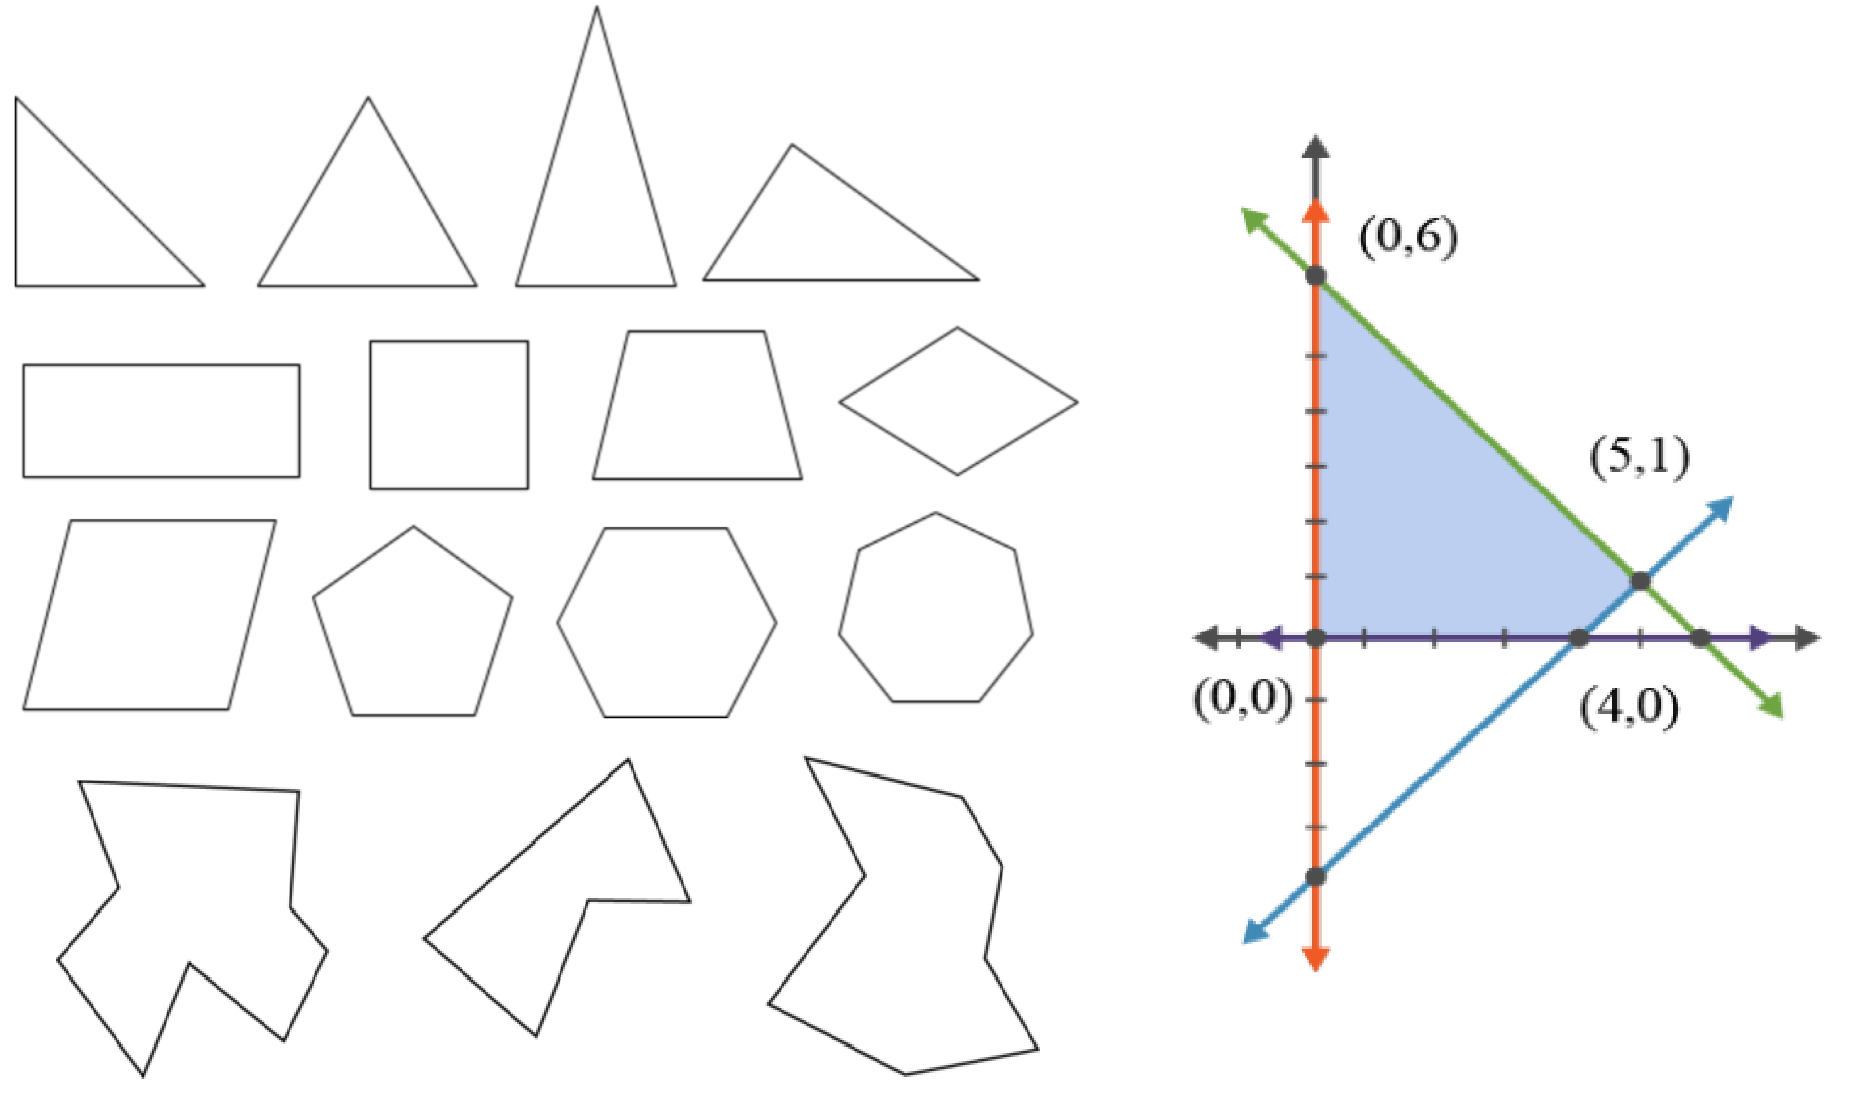
\includegraphics[width=\textwidth]{images/poligonos.png}
    \onslide<5>\centering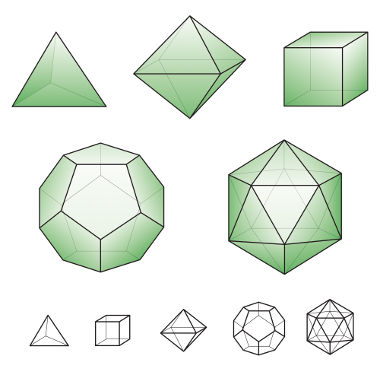
\includegraphics[width=0.70\textwidth]{images/poliedro.jpg}
    \end{overprint}
    
\end{frame}

%% --------------------------------------------------------

\begin{frame}{Politopo convexo}
    Em programação linear, todo politopo é um conjunto convexo
    \begin{itemize}
        \item Espaço afim fechado sobre combinações convexas \href{https://pt.wikipedia.org/wiki/Conjunto_convexo}{\beamergotobutton{Link}} 
    \end{itemize}
    
    \begin{center}
        \animategraphics[autoplay,loop,width=\textwidth]{1}{images/convexidade/convexo-}{0}{2}
    \end{center}
    
\end{frame}

%% --------------------------------------------------------

\begin{frame}{Hipótese da aditividade}
O conceito de aditividade da função objetivo diz que o custo total da função objetivo é a soma das parcelas associadas a cada atividade
\begin{itemize}
    \item O todo é igual a soma de suas partes
\end{itemize}

\vspace{0.5cm}
$$\min \sum_{i = 0}^n c_i x_i$$

\vspace{0.5cm}

Por exemplo, se em 100ml de leite achocolatado encontramos
70mg de cálcio e, em 100g de pão de forma encontramos
2,5mg do mesmo componente, então na refeição composta
por 100ml de leite achocolatado e 100g de pão de forma
ingerimos 72,5mg de cálcio
    
\end{frame}

%% --------------------------------------------------------

\begin{frame}{Hipótese da proporcionalidade}
O custo de cada atividade é proporcional ao nível de operação da atividade

\vspace{0.5cm}

$$\min \sum_{i = 0}^n c_i x_i$$

\vspace{0.5cm}

Por exemplo, 100ml de leite possui 70mg de cálcio
\begin{itemize}
    \item Então, 50ml de leite contém 35mg de cálcio
\end{itemize}

\end{frame}

%% --------------------------------------------------------

\begin{frame}{Hipótese da separabilidade (ou divisibilidade)}
As atividades podem ser divididas em qualquer nível fracionário

\vspace{0.5cm}

$$\min \sum_{i = 0}^n c_i x_i$$

\vspace{0.5cm}

Por exemplo, se uma porção de leite contém 100ml
\begin{itemize}
    \item Você pode servir qualquer fração de uma porção
    \begin{itemize}
        \item 50\% $\rightarrow$ 50ml
        \item ~~0\% $\rightarrow$  0ml
        \item 89\% $\rightarrow$ 89ml
        \item $\ldots$
    \end{itemize}
\end{itemize}

\end{frame}

%% --------------------------------------------------------

\begin{frame}{Hipótese da certeza}
Assume-se que todos os parâmetros do modelo são conhecidos

\vspace{0.5cm}

Problema da dieta:
$$\begin{matrix}
        \min & \sum_{i \in F}~x_i\,c_i\\ 
             & \sum_{i \in F}~x_i\,a_{ij} & \geq m_j, & \forall j \in N \\
             & x_i & \geq 0 & \forall i \in F
        \end{matrix}    
$$
Os parâmetros $a_{ij}$ e $m_j$ devem ser conhecidos
\begin{itemize}
    \item Caso contrário, é impossível montarmos um modelo de otimização linear
\end{itemize}

\end{frame}

%% --------------------------------------------------------

\begin{frame}{Pontos extremos}
Um ponto extremo ocorre no encontro de duas ou mais linhas
\begin{itemize}
    \item No encontro entre duas ou mais restrições
    \item É um vértice
\end{itemize}

\begin{overprint}
\onslide<1>\centering 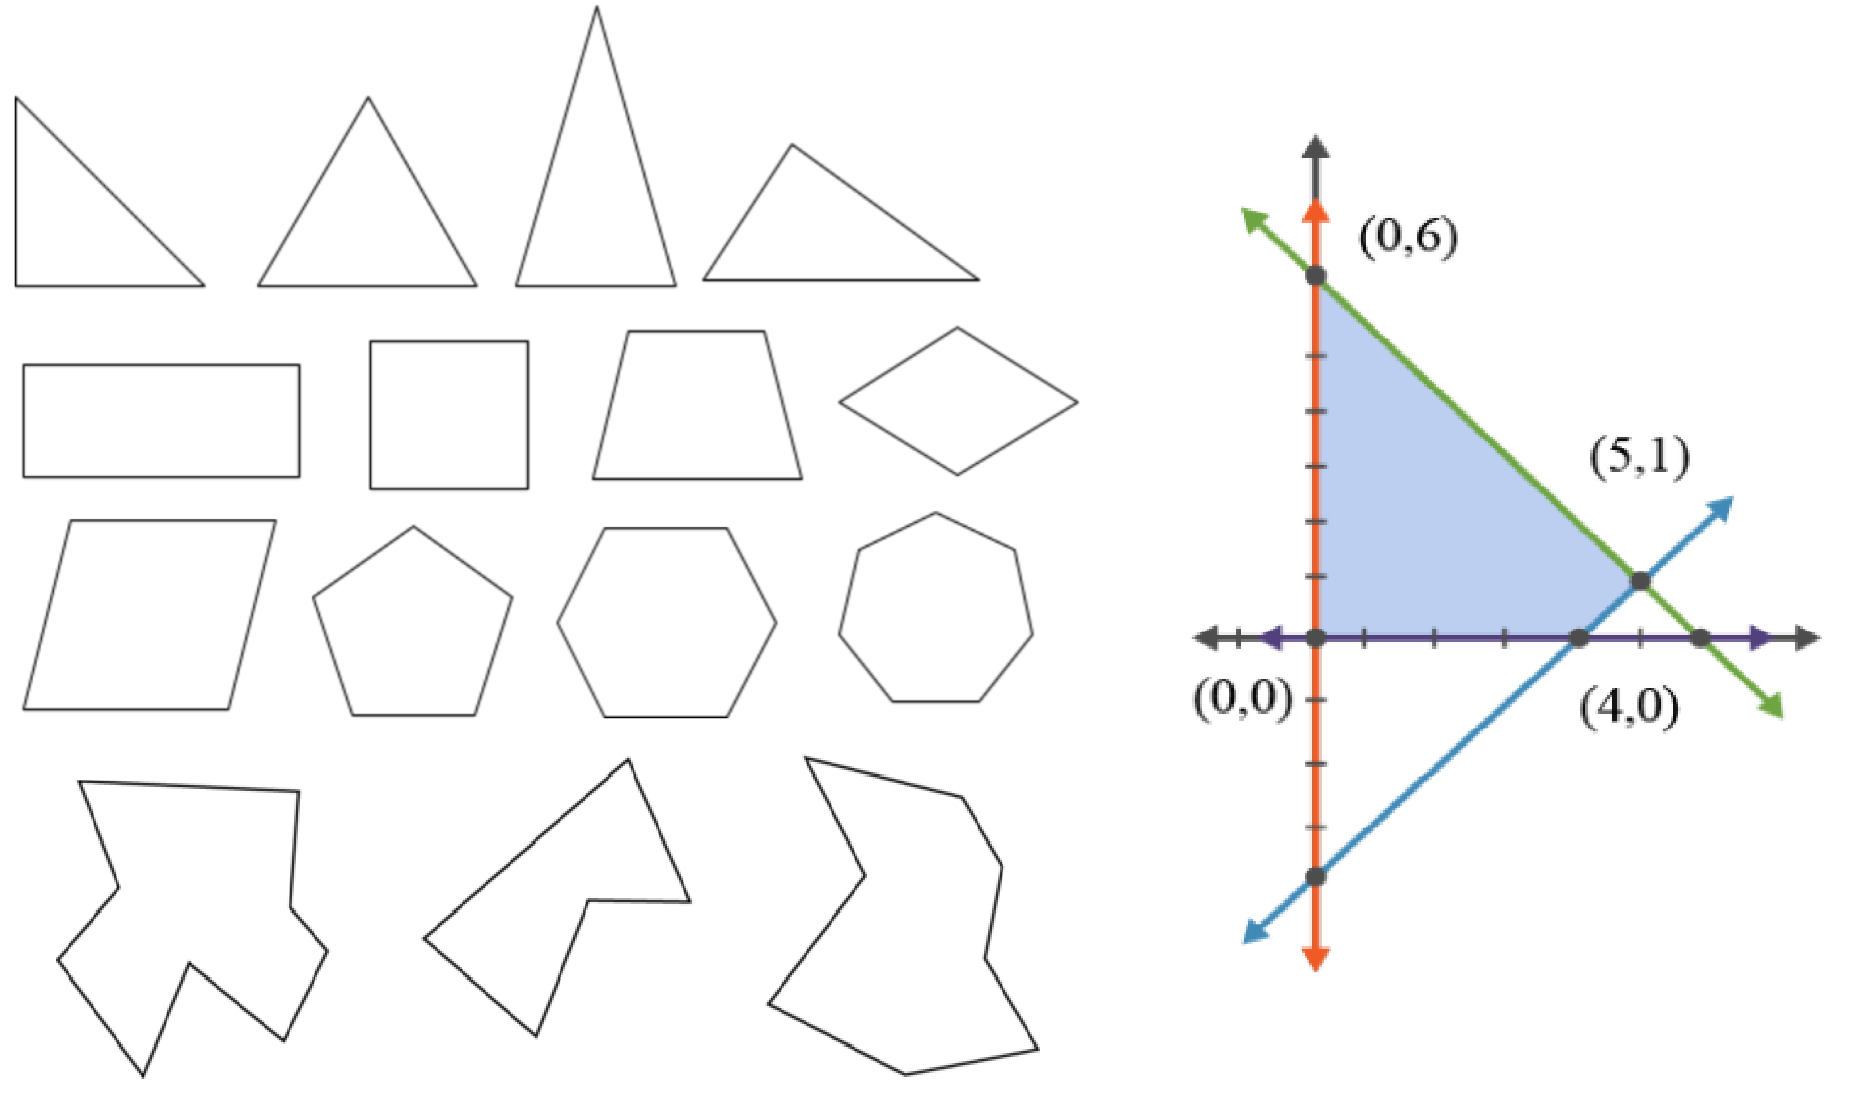
\includegraphics[width=\textwidth]{images/poligonos.png}
\onslide<2>\centering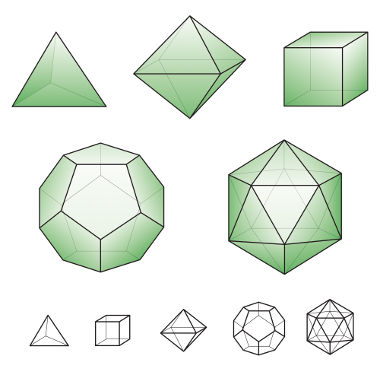
\includegraphics[width=0.60\textwidth]{images/poliedro.jpg}
\end{overprint}

\end{frame}

%% --------------------------------------------------------

\begin{frame}{Teorema fundamental da Programação Linear}

O máximo (ou mínimo) de uma função objetivo linear sob um politopo convexo ocorre em um ponto extremo 

\vspace{0.5cm}

Prova: \href{https://en.wikipedia.org/wiki/Fundamental_theorem_of_linear_programming}{\beamergotobutton{Link}} 

\centering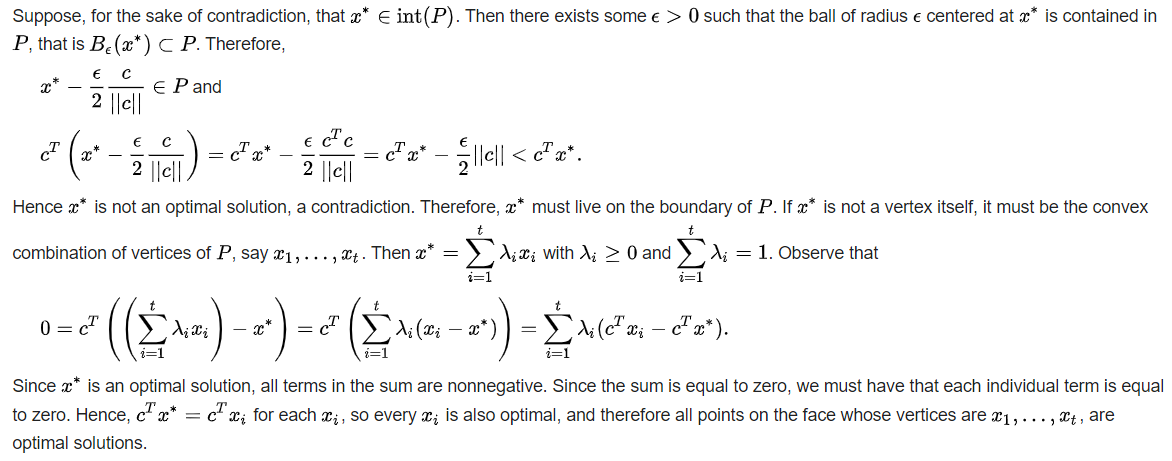
\includegraphics[width=\linewidth]{images/teorema_fundamental.png}

\end{frame}

%% --------------------------------------------------------

\begin{frame}{Conjunto de soluções viáveis é um conjunto convexo}

\begin{columns}[T]
    \begin{column}{.49\textwidth}
    
    \vspace{1cm}
    
    Um conjunto de equações lineares produz um politopo
    \vspace{1cm}    
    
    Soluções viáveis estão dentro deste politopo
    
    \vspace{1cm}    
    
    Portanto, o conjunto é convexo
    \end{column}
    \begin{column}{.49\textwidth}
        \centering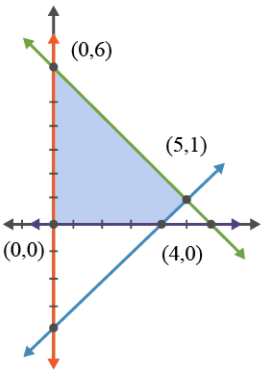
\includegraphics[width=\linewidth]{images/modelo_pl.png}
    \end{column}
\end{columns}

\end{frame}

%% --------------------------------------------------------

\begin{frame}{Politopo tem um número finito de pontos extremos}

Nós ainda não discutimos o tema, mas...
\begin{itemize}
    \item Pode-se representar os coeficientes de problema de programação linear utilizando uma matriz bi-dimensional
    \begin{itemize}
        \item Cada linha representa uma restrição ($m$)
        \item Existe uma coluna para cada variável do problema ($n$)
        \item O valor de cada célula representa o coeficiente de uma variável em uma restrição
    \end{itemize}
\end{itemize}

\vspace{0.5cm}

O número máximo de pontos extremos em um politopo convexo é

$$\frac{n!}{m!(n-m)!}$$

\end{frame}

%% --------------------------------------------------------

\begin{frame}{Modelos de programaçao linear sem solução}

Modelos mal construídos podem não ter nenhuma solução
\begin{itemize}
    \item Não é possível construir um politopo
    \item Em Algebra Linear, dizemos que é um sistema impossível (SI)
\end{itemize}

\vspace{0.5cm}

$$\begin{matrix}
        \max & x + y + z\\ 
             & x + y & \geq 5 \\
             & x + z & \geq 5 \\
             & x + y + z & \leq 4 \\
             & x & \geq 0 \\
             & y & \geq 0 \\
             & z & \geq 0
        \end{matrix}    
$$

\end{frame}

%% --------------------------------------------------------

\begin{frame}{Modelos com solução ótima não conhecida}

Sistema Possível e Indeterminado (SPI)

\vspace{1cm}

\begin{columns}[T]
    \begin{column}{.49\textwidth}
    \vspace{1cm}
    $$\begin{matrix}
        \max & x + y \\ 
             & x + y & \geq 2 \\
             & x & \geq 0 \\
             & y & \geq 0 
        \end{matrix}    
$$
    \end{column}
    \begin{column}{.49\textwidth}
        \centering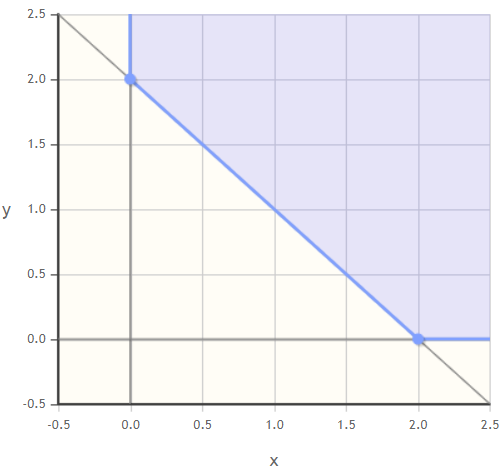
\includegraphics[width=\linewidth]{images/nao_conhecida.png}
    \end{column}
\end{columns}

\end{frame}

%% --------------------------------------------------------

\begin{frame}{Modelos com múltiplas soluções ótimas}

Sistema Possível e Indeterminado (SPI)

\vspace{1cm}

\begin{columns}[T]
    \begin{column}{.49\textwidth}
    \vspace{1cm}
    $$\begin{matrix}
        \max & x + y \\ 
             & x + y & \leq 5 \\
             & x & \geq 0 \\
             & y & \geq 0 
        \end{matrix}    
$$
    \end{column}
    \begin{column}{.49\textwidth}
        \centering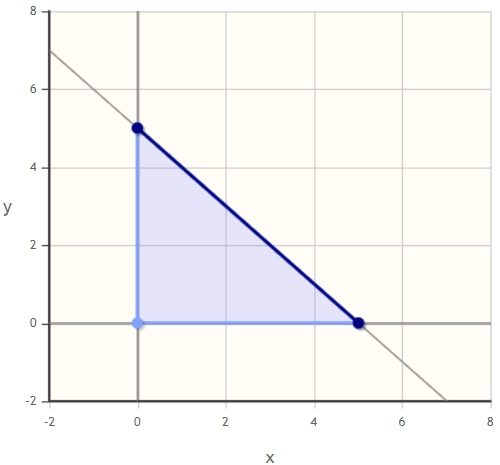
\includegraphics[width=\linewidth]{images/multiplas_solucoes.png}
    \end{column}
\end{columns}

\end{frame}

\end{document}